% --- C L O U D   C O M P U T I N G ---

Cloud Computing ist aus der heutigen Zeit nicht mehr wegzudenken. Täglich entstehen enorme Datenmengen, die gespeichert, verarbeitet und abgerufen werden müssen. Immer mehr Menschen und Unternehmen nutzen die Vorteile des Internets, um unabhängig von Standort und Uhrzeit auf bestimmte Dienste zuzugreifen. Von einfachen Ablagen in der Cloud bis hin zu Social-Media-Plattformen wie Instagram und Facebook wird alles mithilfe von Cloud Computing umgesetzt.

Besonders für Unternehmen ergeben sich dadurch völlig neue Möglichkeiten. Insbesondere die Software-Auslieferung hat sich grundlegend verändert. 
Software-Releases müssen nicht mehr Monate im Voraus geplant werden, sondern können dank neuer Technologien innerhalb weniger Minuten oder sogar Sekunden erfolgen.\\
\cite{EA:Web59}

All dies wäre ohne die Cloud undenkbar. Im Folgenden soll der Begriff Cloud Computing näher beschrieben werden.


    % --- D E F I N I T I O N ---

    \subsection{Definition}

    Die Cloud besteht aus einem großen Netzwerk von Servern, die auf der ganzen Welt verteilt sind und miteinander kommunizieren.
    Dabei ist es möglich, IT-Ressourcen, die in einem Rechenzentrum betrieben werden, zu mieten (siehe Abbildung \ref{fig:cloud-computing}). 
    
    Beispiele für solche Ressourcen sind:
    \begin{itemize}
        \item Server
        \item Speicher
        \item Datenbanken
    \end{itemize}

    Dies bietet den Vorteil, dass kein Geld für die Anschaffung von Hardware investiert werden muss. Bei Cloud Computing gibt es keine allgemein festgelegte Architektur. Es gibt mehrere Cloud-Modelle, die genutzt werden können, um die Wünsche der Kund/innen zu erfüllen.
    Diese werden in Abschnitt \ref{Cloud-Modelle} näher erläutert.
    \cite{EA:Web55}
    
    \begin{figure}[H]
        \centering
        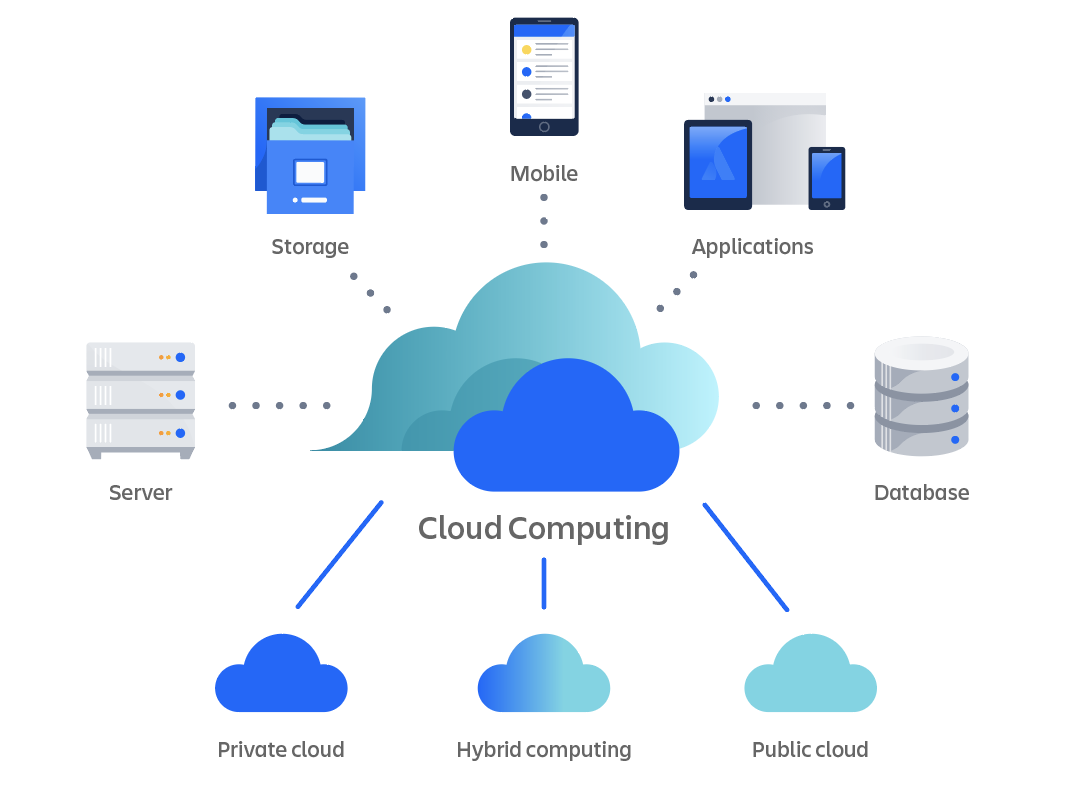
\includegraphics[width=0.75\linewidth]{images/EA/cloud-computing.png}
        \caption{Cloud Computing \\ \cite{EA:Web55}}
        \label{fig:cloud-computing}
    \end{figure}


    % --- C L O U D   -   M O D E L L E ---
    
    \subsection{Cloud-Modelle} \label{Cloud-Modelle}

        Grundsätzlich kann zwischen drei verschiedenen Arten von Cloud-Computing unterschieden werden:
        \begin{itemize}
            \item Public Cloud
            \item Private Cloud
            \item Hybrid Cloud
        \end{itemize}

    
        % --- P U B L I C   C L O U D ---
    
        \subsubsection{Public Cloud}
    
        Bei diesem Cloud-Computing-Modell sind die gesamten Ressourcen im Besitz des Cloud-Serviceanbieters. 
        Diese Cloud-Dienste können je nach Anbieter kostenlos oder kostenpflichtig sein und sind über das Internet erreichbar.
        Außerdem können die Ressourcen so ausgewählt werden, dass sie auf unterschiedliche Anwendungsfälle zugeschnitten werden können. Der/die Nutzer/in 
        wählt dabei einfach die benötigten Ressourcen über eine Benutzeroberfläche aus und kann somit innerhalb kürzester Zeit Software ausliefern. Alle zusätzlichen Aufgaben, wie die Bereitstellung und Verwaltung, werden vom Cloud-Anbieter übernommen. Der Einsatz spezieller Werkzeuge kann den Prozess der Systembereitstellung in der Cloud beschleunigen. Einige dieser Werkzeuge werden in Abschnitt \ref{IaC} näher beschrieben.
        \cite{EA:Web53, EA:Web54}
    
        Zu den bekanntesten Anbietern gehören:
        \begin{itemize}
            \item Amazon Web Services (AWS)
            \item Google Cloud
            \item Microsoft Azure
        \end{itemize}
    
        % --- P U B L I C   C L O U D   -   P R O S   &   C O N S ---
    
        \textbf{Vor- und Nachteile der Public Cloud}
    
        Zudem gibt es weitere Vorteile, die durch die Verwendung einer Public Cloud geschaffen werden können.
        Beispielsweise können die \textbf{Infrastrukturkosten gesenkt} werden, da keine Betriebskosten für einen lokal installierten Server mehr anfallen. Stattdessen wird nur noch für die tatsächlich genutzten Ressourcen in der Cloud bezahlt. Durch die flexible Verwaltung von Ressourcen ist auch die \textbf{Skalierung} unproblematisch. 
    
        Allerdings hat auch die Public Cloud ihre Schattenseiten, die berücksichtigt werden müssen. Speziell dann, wenn es um den Umgang mit sensiblen Daten geht, ist besondere Vorsicht geboten, da eine \textbf{unzureichende Konfiguration} zu \textbf{Sicherheitslücken} führen kann.
        Darüber hinaus muss sichergestellt werden, dass \textbf{stets eine stabile Internetverbindung besteht}, damit die in der Cloud bereitgestellten Dienste auch jederzeit erreicht werden können. \cite{EA:Web53} \\

        % --- E I N S A T Z G E B I E T E   -   P U B L I C   C L O U D ---
    
        \textbf{Einsatzgebiete der Public Cloud}
    
        Durch die zahlreichen Möglichkeiten, die Public Clouds bieten, können diese für extrem unterschiedliche Anwendungsfälle eingesetzt werden.
        Allgemein gesagt, eignet sich die Public Cloud besonders für Softwarelösungen, bei denen die genaue Auslastung vorab schwer abgeschätzt werden kann und/oder sich die Anforderungen im Laufe des Projekts häufig verändern.
        \cite{EA:Web53}

        \clearpage
        
    
        % --- P R I V A T E   C L O U D ---
    
        \subsubsection{Private Cloud}
    
        Da die Public Cloud trotz ihrer zahlreichen Vorteile nicht für jeden Anwendungsfall geeignet ist, gibt es weitere Arten von Cloud Computing, die in Betracht gezogen werden können. Eine davon ist die \textbf{Private Cloud}. 
    
        Der wesentliche Unterschied zur Public Cloud ist, dass die \textbf{Cloud-Computing-Ressourcen nicht mit anderen Personen geteilt} werden, sondern ausschließlich für Personen mit entsprechenden Zugriffsrechten zugänglich sind.
        
        Dies wird in Abbildung \ref{fig:private-cloud-vs-public-cloud} veranschaulicht:
        \begin{figure}[H]
            \centering
            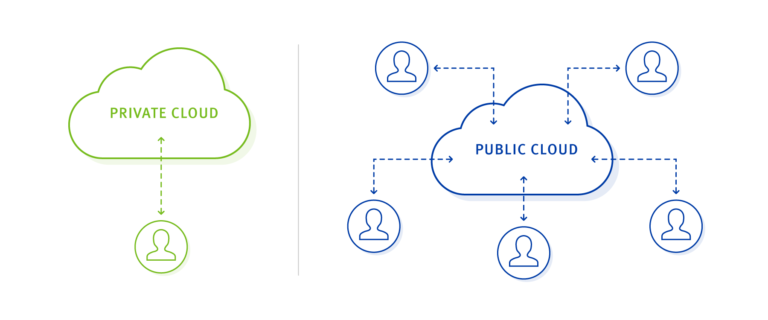
\includegraphics[width=0.85\linewidth]{images/EA/private-cloud-vs-public-cloud.png}
            \caption{Private Cloud vs. Public Cloud \\ \cite{EA:Img01}}
            \label{fig:private-cloud-vs-public-cloud}
        \end{figure}
    
        Zudem kann die Private Cloud weiter spezifiziert werden:
        \begin{itemize}
            \item \textbf{Lokale Private Cloud}
            \begin{itemize}[label=$\circ$]
                \item IT-Infrastruktur befindet sich am Standort des Kunden
                \item Bereitstellung \& Verwaltung erfolgt intern
            \end{itemize}
            \item \textbf{Cloud-Dienstanbieter}
            \begin{itemize}[label=$\circ$]
                \item Rechenressourcen werden in einem externen Rechenzentrum betrieben
                \item Ein Drittanbieter übernimmt die Bereitstellung und Verwaltung
            \end{itemize}
        \end{itemize}
    
        Verfügt ein Unternehmen über qualifiziertes Personal, das sich um die lokal installierte IT-Infrastruktur kümmert, kann auf externe Anbieter
        verzichtet werden. Ist dieses Kriterium nicht gegeben, so ist es wirtschaftlich sinnvoller, diese Aufgaben an einen Cloud-Dienstanbieter auszulagern, um die Anforderungen der Kundschaft effizient zu erfüllen.
        \cite{EA:Web54} \\
    
        % --- P R I V A T E   C L O U D   -   P R O S   &   C O N S ---
    
        \textbf{Vor- und Nachteile der Private Cloud}
    
        Dadurch, dass die Private Cloud eine isolierte Umgebung ist, auf die fremde Personen und Unternehmen keinen Zugriff haben, bietet diese Art von Cloud Computing einige Vorteile in Bezug auf \textbf{Sicherheit und Kontrolle}.
        Die Ressourcen können so angepasst werden, dass sie den Anforderungen der Auftraggebenden entsprechen.
    
        Wie die Public Cloud hat auch die Private Cloud ihre Nachteile. Um die möglichen Probleme der Private Cloud aufzuzeigen, wirft man einen Blick auf das Projekt CGM MAXX LITE. Wie in Abschnitt \ref{Projektbezug - Anforderungsanalyse} beschrieben, handelt es sich bei diesem Projekt um die Entwicklung einer Arztsoftware. Da diese Anwendung mit sehr sensiblen Daten arbeitet, die aus datenschutzrechtlichen Gründen nicht von unbefugten Personen eingesehen werden dürfen, ist die Private Cloud eine gute Lösung. 
    
        Sollte ein Arzt die Software erwerben und On-Premise\footnote{Software vor Ort betreiben} betreiben wollen, dann muss dafür eine \textbf{entsprechende Infrastruktur angeschafft und konfiguriert} werden, was erstens sehr \textbf{kostspielig} sein kann und \textbf{zusätzlichen Wartungsaufwand} erfordert. Zudem ist die Infrastruktur weniger flexibel als bei einem Drittanbieter, was im schlimmsten Fall zu Engpässen führen kann.
        \cite{EA:Web56} \\
    
    
        \textbf{Einsatzgebiete der Private Cloud}
    
        Wie aus dem obigen Absatz hervorgeht, eignet sich der Einsatz einer privat betriebenen Cloud besonders dann, wenn in etwa abgeschätzt werden kann, wie viele Ressourcen benötigt werden, um die Hardware gezielt auszuwählen und einen reibungslosen Betrieb des Softwaresystems zu gewährleisten. Auch für Anwendungen, bei denen ein hohes Maß an Sicherheit erforderlich ist, eignet sich dieses Cloud-Computing-Modell hervorragend.
    
        Weitere Beispiele wären Anwendungen in folgenden Bereichen:
        \begin{itemize}
            \item Finanzen
            \item Recht
            \item Politik
        \end{itemize}
    
        \cite{EA:Web56}
        
        \clearpage
    
    
        % --- H Y B R I D   C L O U D ---
    
        \subsubsection{Hybrid Cloud}
    
        Die letzte Art des Cloud Computings, die in dieser Arbeit beschrieben wird, ist die \textbf{Hybrid Cloud}. 
        Im Vergleich zu den zuvor erläuterten Cloud-Modellen kommen hier mehrere unterschiedliche Clouds zum Einsatz. 
        Es handelt sich also um eine \glqq{Mischform}\grqq\ bestehend aus Public und Private Cloud (siehe Abbildung \ref{fig:hybrid-cloud}).
    
        Die Clouds werden dabei so miteinander verbunden, dass Daten ausgetauscht werden können. Werden mehrere Clouds derselben Art (z.B. zwei öffentliche Clouds) eingesetzt, so spricht man von einer \textbf{Multi Cloud}.
    
        \begin{figure}[H]
            \centering
            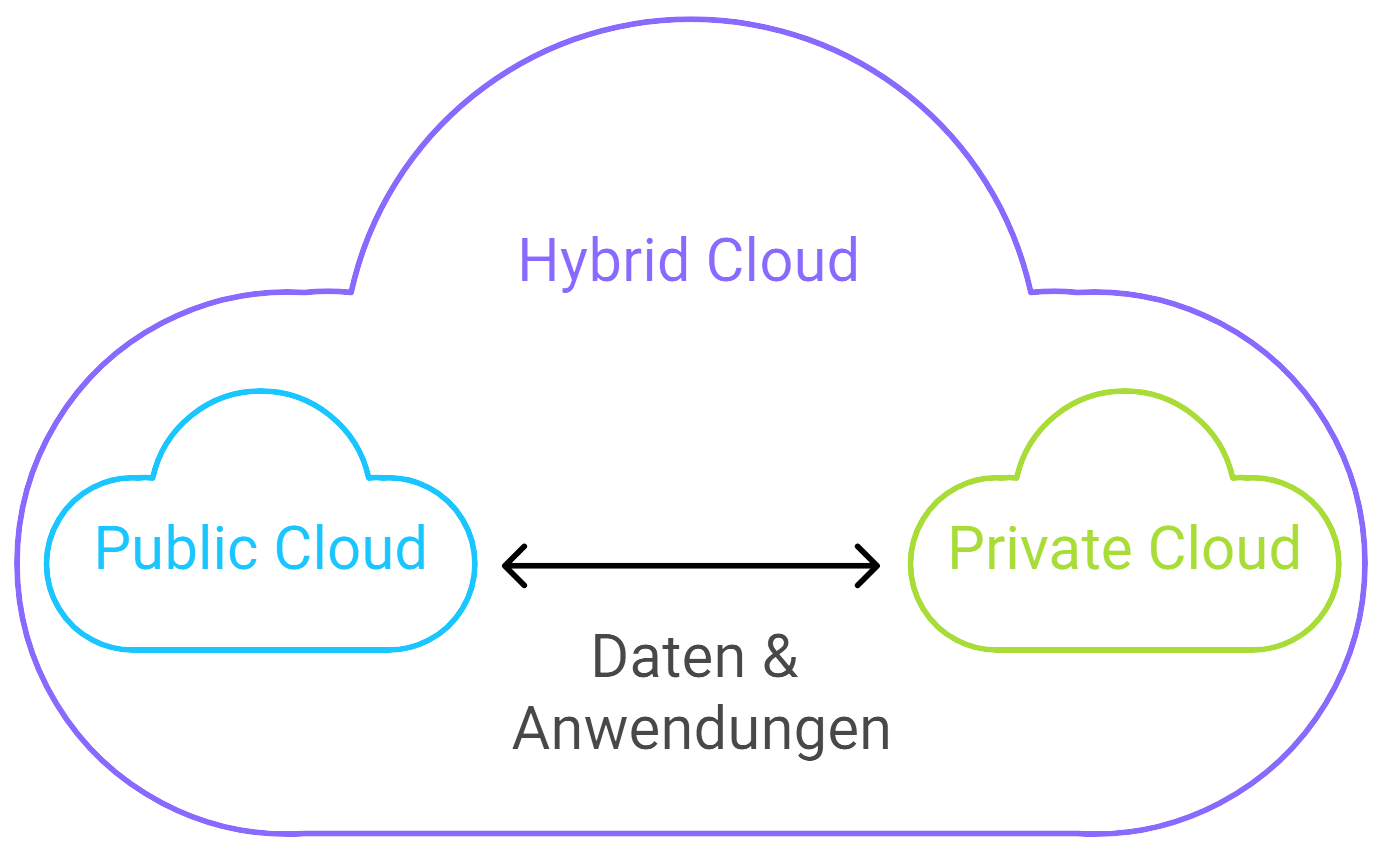
\includegraphics[width=0.6\linewidth]{images/EA/hybrid-cloud.png}
            \caption{Hybrid Cloud}
            \label{fig:hybrid-cloud}
        \end{figure}
    
        Speziell bei Anwendungen, bei denen ein großer Wert auf Datenschutz gelegt wird und worauf viele verschiedene Personen zugreifen können, ist es wichtig, die Daten sicher zu verwalten. In solchen Fällen ist es meist nicht mehr ausreichend, auf ein einziges Cloud-Modell zu vertrauen, weswegen immer häufiger auf hybride Cloud-Lösungen gesetzt wird.
         \cite{EA:Web57} 
    
         Um auf das zuvor genannte Beispiel zurückzukommen, das erklärt, wofür sich eine private Cloud besonders eignet, folgt nun eine kurze Ergänzung in Bezug auf die hybride Cloud:
    
        Arbeitet eine Applikation mit sensiblen Daten, so ist es sinnvoll, diese lokal oder in einer privat verwalteten Cloud abzulegen, während öffentlich zugängliche Dienste in der Public Cloud bereitgestellt werden sollten, um einen schnellen und einfachen Zugriff zu gewährleisten. 
    
        \clearpage
    
        \textbf{Vor- und Nachteile der Hybrid Cloud}
    
        Eine gezielte Kombination verschiedener Cloud-Umgebungen ermöglicht eine effizientere Ressourcennutzung, steigert die Flexibilität und kann Sicherheitsanforderungen besser erfüllen. Je nachdem, was betrieben werden soll, eignet sich eine Lösung besser als die andere. 
    
        Trotz der Vorteile beider Cloud-Modelle bringt die Hybrid Cloud auch neue Herausforderungen mit sich.
        Ein Nachteil ist beispielsweise ein erhöhter Aufwand in Bezug auf Verwaltung und Konfiguration. Grund dafür sind die vielen beteiligten Komponenten, die miteinander interagieren und im Auge behalten werden müssen. \cite{EA:Web58}
    